\section{Problem Setting and Dataset}

\subsection{Problem setting}

Our dataset composed mobile data access records of a set of users. Each user has a set of records $R = {r_1, r_2, ...,r_i, ... r_n}$ which has already been sorted by time stamp.
Each mobile data access record $r$ has the following fields:
\begin{equation*}
  \langle UserID, TowerLocation, TimeStamp, DataAccess, \dots \rangle
\end{equation*}
where
\begin{itemize}
  \item $UserID$ is identifier of a user, a hashed value for anonymity
  \item $TowerLocation$ is the location (latitude and longitude) of cell phone tower with witch the user communicated, denoted by $l$
  \item $TimeStamp$ is the time stamp of a mobile data access record, denoted by $t$
  \item $DataAccess$ is the mobile data access of the app for this records, including app identifier and data volume, denoted by $DA$
  \item ... represents many other attributes not of focus here.
\end{itemize}
We would like to estimate speed $s$ of users by analyzing location information $l$ in their mobile data access records $R$, and find the correlations of $s$ and $DA$. 

\subsection{Dataset Description}

\begin{figure*}[ht]
  \centering
  \subfigure[Distribution of number of records]{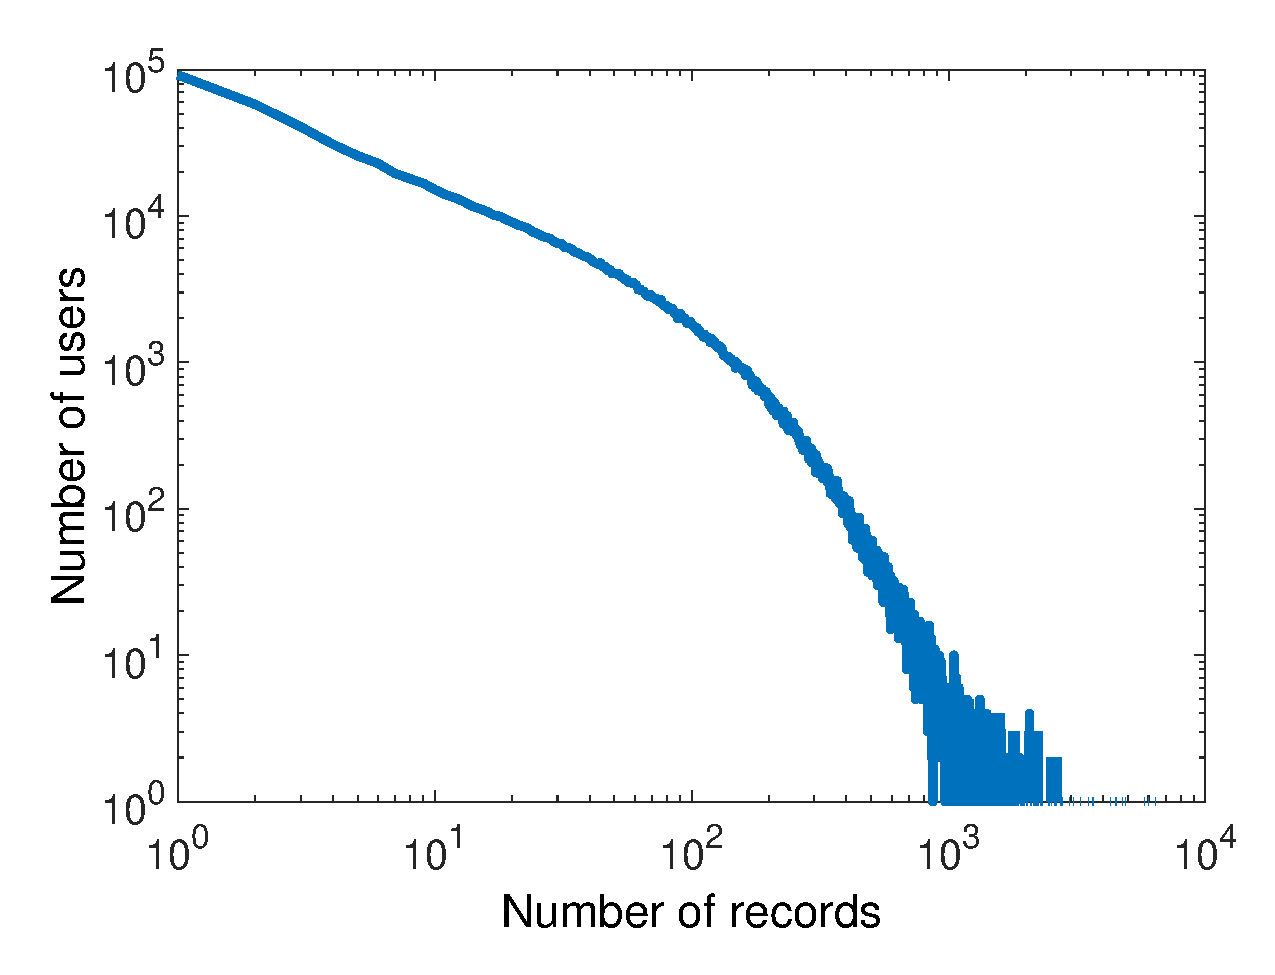
\includegraphics[width=0.32\textwidth]{figures/record_count_hist.pdf}}
  \subfigure[Distribution of time interval]{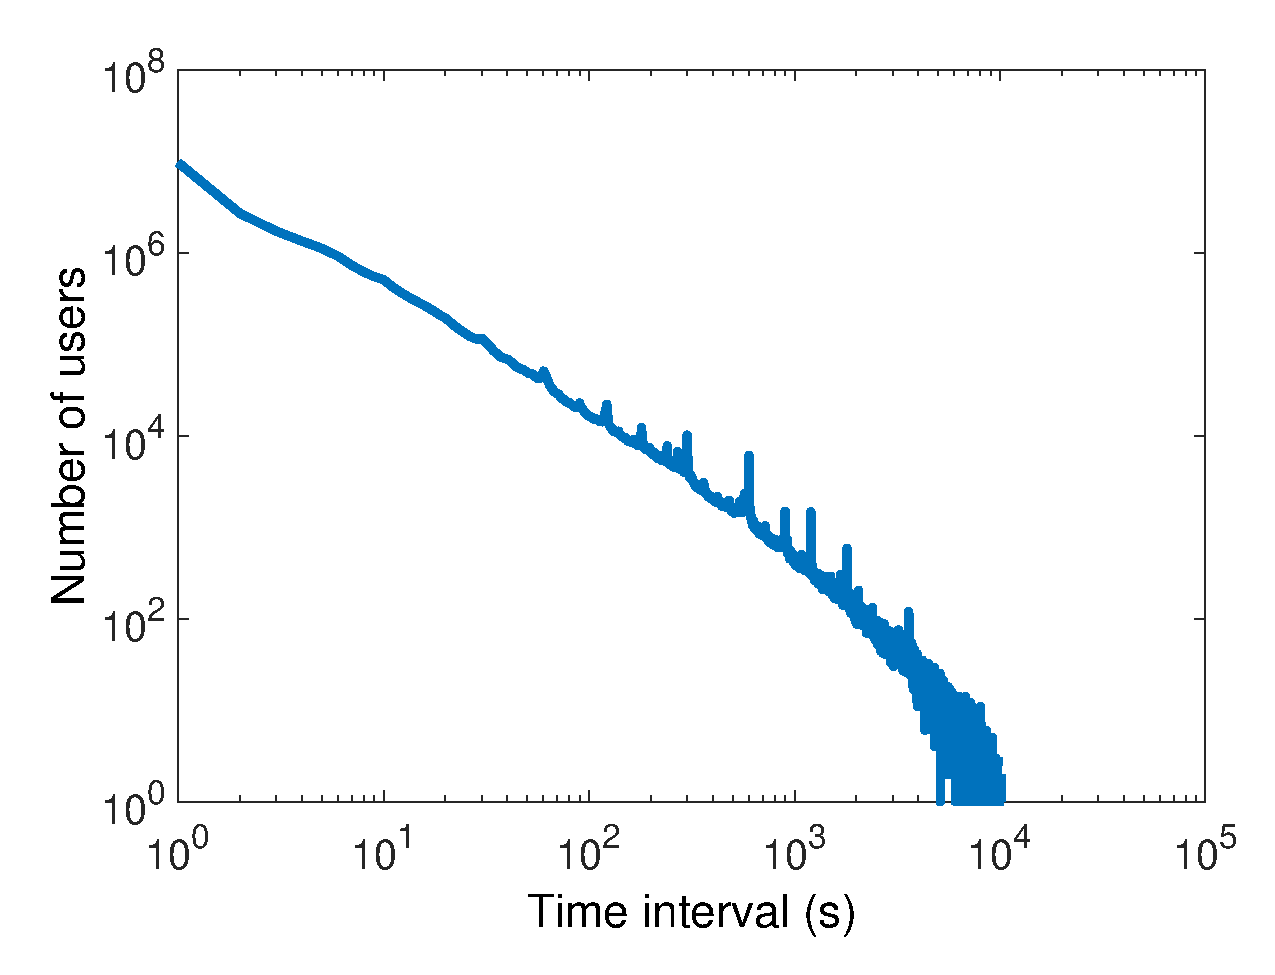
\includegraphics[width=0.32\textwidth]{figures/time_interval_hist.pdf}}
  \subfigure[Distribution of visited towers]{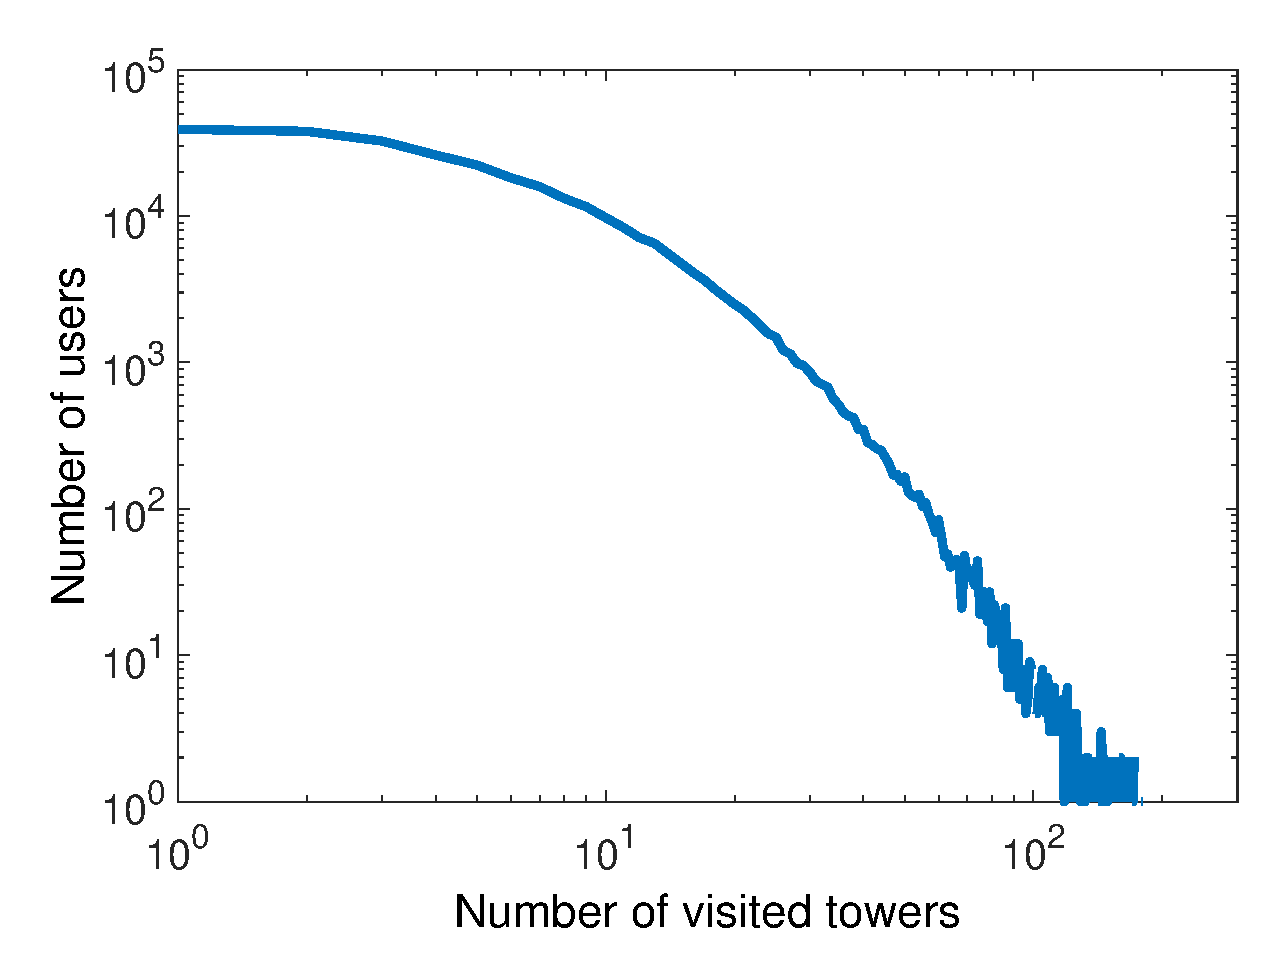
\includegraphics[width=0.32\textwidth]{figures/visited_tower_hist.pdf}}
  \caption{dataset statistics}
	\label{fig:data_stat}
\end{figure*}

The dataset is mobile data access records provided by a cellular network operator in China. It was collected from three cities (xuzhou, yancheng and taizhou), including both urban and suburban area, during a three-hour period in the early evening (6pm - 9pm). The dataset includes more than 58 million mobile data access records with a total volume of more than 720 gigabytes, which covers all cell phones that were actively exchanging data with 5199 cell towers in three cities during the observation period. The number of unique users included in this dataset is 0.9 million. And the total active time of all user is more than 1 million hours. Note that the available number of mobile data access records for each user is far from even. We show in Fig.~\ref{fig:data_stat} the distribution of number of data access records per user in log-log scale.

\subsubsection{App category information}

According to the mobile service provider, all apps in our trace are grouped into 19 categories. We showed the name, the number of apps and total volume in our data trace of each category in Table~\ref{table:appcat}.  

\begin{table}
	\centering
	\begin{tabular}{ccc}\hline
	App category & number of apps & data volume (GB) \\ \hline
	Instant Messages & 30 & 97.3\\
	Reading & 101 & 17.6\\
	Microblog & 43 & 13.0\\
	Navigation & 38 & 10.8\\
	Video & 63 & 45.2\\
	Music & 33 & 27.4\\
	App market & 45 & 37.0\\
	Game & 106 & 9.2\\
	Online payment & 18 & 1.2\\
	Comic & 12 & 0.8\\
	Email & 10 & 1.5\\
	P2P & 8 & 3.9\\
	VOIP & 17 & 0.3\\
	Multimedia Messages & 2 & 0.3\\
	Browser \& Download & 558 & 353.5\\
	Finance & 25 & 0.7\\
	Security & 22 & 5.2\\
	Other1 & 237 & 74.7\\
	Other2 & 7 & 21.1\\ \hline
	\end{tabular}
	\caption{App categories}
	\label{table:appcat}
\end{table}

\subsubsection{An example user's trace}

\begin{figure}[h]
    \centering
    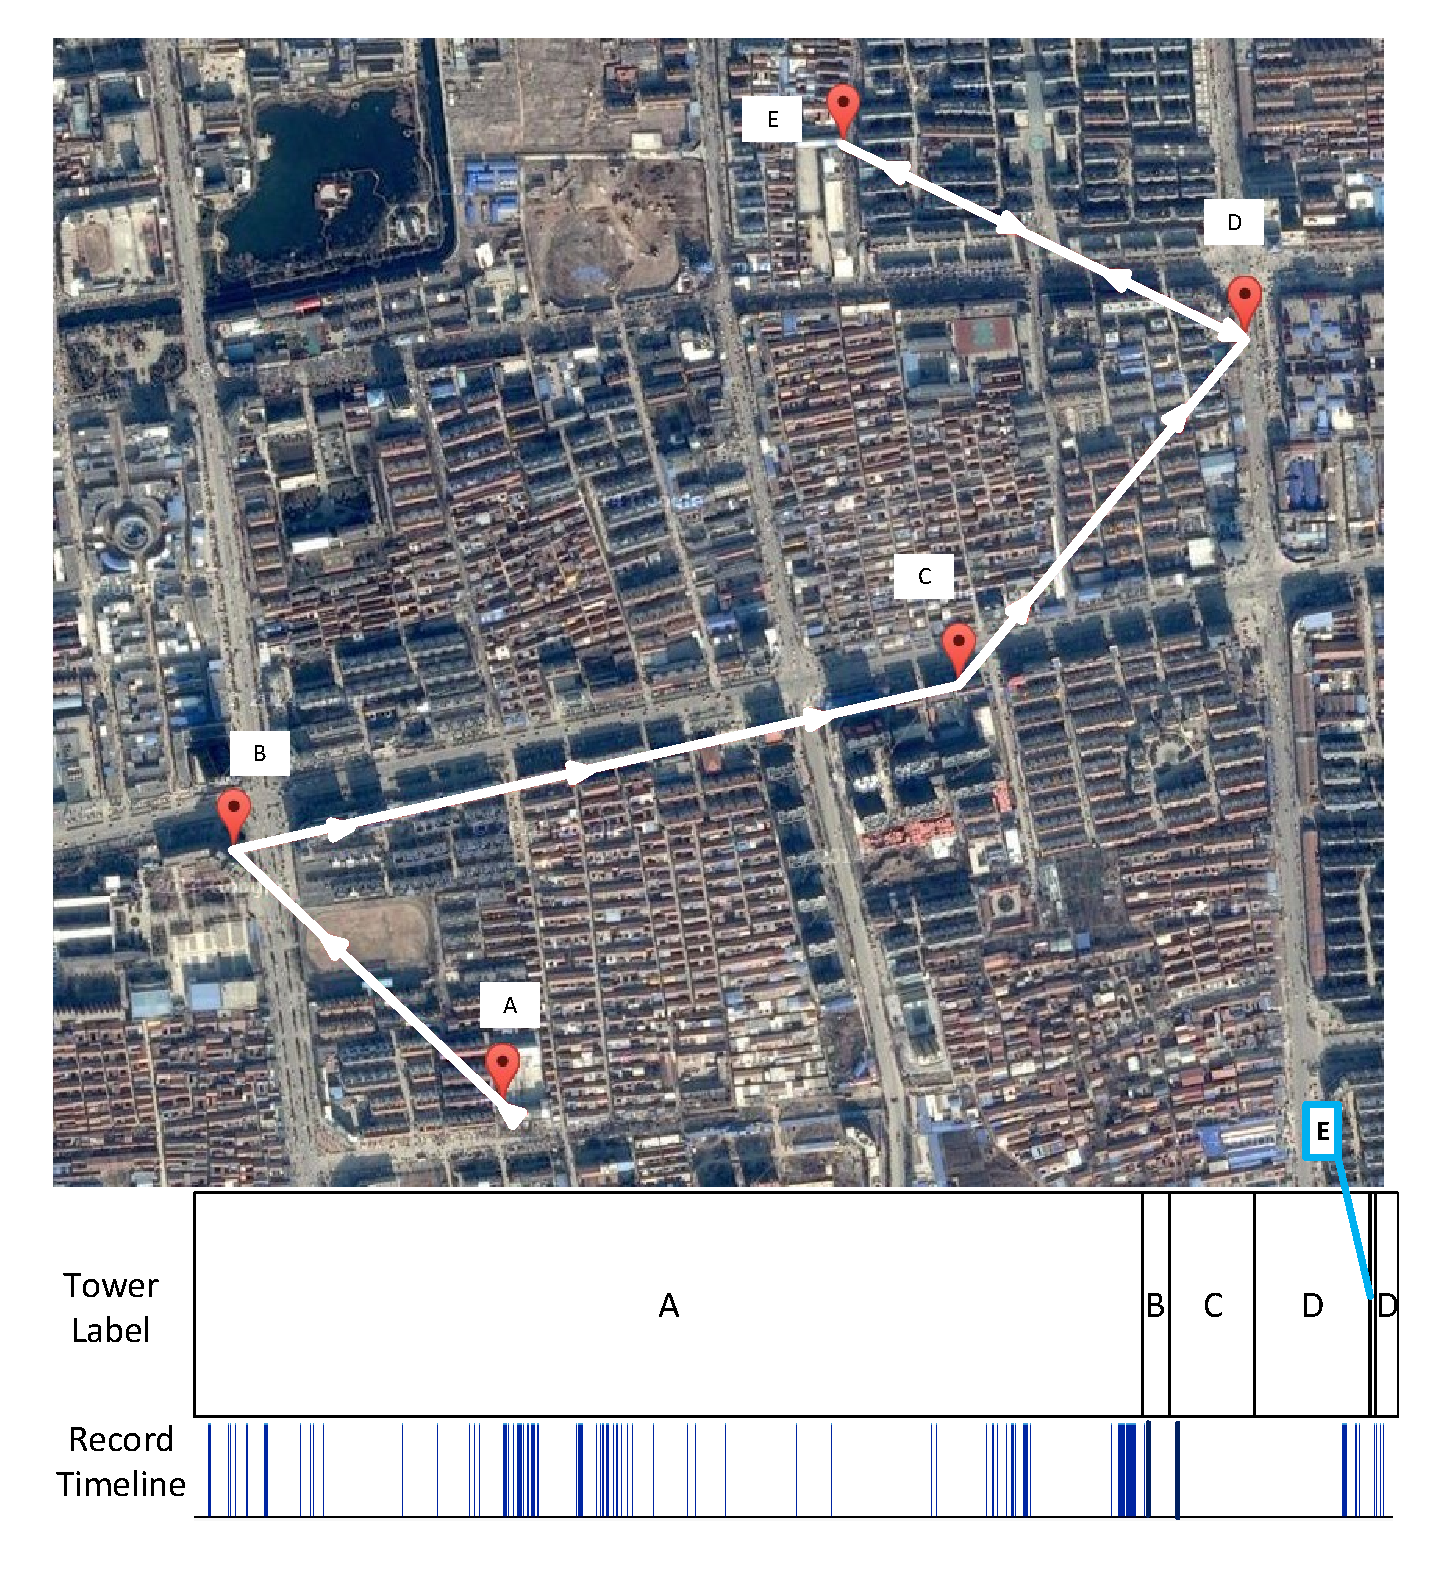
\includegraphics[width=\linewidth]{./figures/typical_user.pdf}
    \caption{A typical data access session of a user.}
    \label{fig:typical_user}
\end{figure}

To give readers a better understanding of our trace and to serve as a running example, we have selected a random user from the dataset and show his mobile data access trace in fig.~\ref{fig:typical_user}. The figure contains two parts. The top part is a map shown the towers that were visited by the user. We use marks to show tower locations and arrowed lines to show the sequence of visiting. The bottom part of the figure shows the time line of the user's data access records with pulses, each pulse represent a mobile data access record and its location on the time line shows its relative time when the mobile data access happens. We also show to which tower the user is communicated for each mobile data access with tower labels above the pulses. So for this particular user, he communicate with tower A for a quite long time, and shortly connected to tower B and then swithed to tower C. After a while, the user was found communicate with tower D. After stayed in tower D's coverage area for a while, he connected to tower E for a very short time, and then switch back to tower D.